%% ----------------------------------------------------------------
%% Methods.tex
%% ---------------------------------------------------------------- 
\chapter{Methods} \label{Chapter: Methods}

%Parameters are defined in Results (not in Methods)

%It doesn't matter if you don't include all the methods, only the ones for the final results.

%Check that you provide enough background information: your reader does not know what you know. Assuming that your reader knows much more than you and therefore omitting background information is a very common problem with students. A typical example would be a Methods section that directly launches into what you have done without first telling why. Although it is evident to you that to get from A to B you need to do X, this is probably far less obvious to the reader. If you only tell the reader that you did X, she is confused. Why did you do X? Never assume that the reader knows your motivation, or the details of every method you used, or why your research question is important. Tell her.

%Plagiarism: use of code (this includes open source code!) that was not written by you, without acknowledgement of the source

%Check that the reader can replicate your results. Verify that your Methods section (and the supplementary sections if any) contains everything that the reader needs to know. Also check that you provide links to your code and your data if it can be released without violating anyone’s privacy.

%\begin{enumerate}
%\item How am I going to measure it?
%\item How am I going to prove it?
%\end{enumerate}


\section{Dataset}
"The dataset used for this coursework is the one produced by Zhou \textit{et al}~\cite{Zhou2014}\footnote{https://www.princeton.edu/\~7Ejzthree/datasets/ICML2014/} for the secondary protein structure prediction problem. There are two different sets within it, one for the purpose of training and the other for testing performance.

The training set is based on the protein sequences from the PISCES server\footnote{http://dunbrack.fccc.edu/Guoli/PISCES\_OptionPage.php}, after being filtered in order to delete similar sequences to the the test set, leading to a size of 5534 sequences. The test set is based on the CB513 dataset \cite{Avdagic2009}. Each sequence contains up to 700 amino acid residues encoded as one-hot vectors, with 20 possible types. Profile information for each amino acid is also included. The secondary structure labels per amino acid correspond to the eight DSSP Q8 classes \cite{Kabsch1983}, 3 for the $\alpha$-helix, 2 for the $\beta$-sheet, and 3 for the coil." [My homework]

\subsection{CullPDB53}
CullPDB (Wang and Dunbrack, 2003)
6125 proteins
"The CullPDB dataset was constructed before CASP10 (i.e., May 2012) and any two proteins in this set share less than 25\% sequence identity with each other." \cite{Wang2016}

"The CullPDB data set from Zhou and Troyanskaya, (2014) was constructed before January 2014, and any two proteins in this set shared less than 25\% sequence identity with each other. This CullPDB contained 6128 proteins. The filtered data set of this CullPDB had a sequence identity of less than 25\% with the CB513 test data, and it contained 5534 protein sequence after filtering." \cite{Fang2017}

"We trained all neural networks on the cullpdb+profile\_6133\_filtered dataset (http://www.princeton.edu/~jzthree/datasets/ICML2014/). [...] The dataset consists of amino acid sequences of proteins with a length up to 700 amino acids and corresponding sequence profiles. [...] The original training set consists of 6133 sequences, but was been filtered to remove sequences that shared more than 30\% identity with sequences in the CB513 dataset." \cite{Jurtz2017}

"We use two publicly available benchmark datasets, pre-processed by Zhou \&Troyanskaya (2014)∗: CullPDB and CB513. Each of these consists of protein sequences and structure label assignments downloaded from the Protein Data Bank archive (PDB) (Berman, Henrick, \& Nakamura, 2003). [...] The full CullPDB dataset contains 6,128 proteins with less than 30\% sequence identity. Here, we use a subset of these data, which has been filtered to reduce sequence identity with the CB513 test data to at most 25\%. The resulting subset consists of 5,534 protein sequences–or equivalently 1,183,318 individual amino acid residues– for prediction. Consistent with Sønderby \& Winther’s (2014) arrangement, we randomly divide these 5,534 proteins into a training set of 5,278 proteins and a validation set of 256 proteins." \cite{Busia2017}
\subsection{CB513 \& CB6133}
"Experimental results on the CB6133 dataset, the public CB513 benchmark" \cite{Li2016}

"CB513 benchmark used in Zhou and Troyanskaya (2014), Wang et al. (2016), Li and Yu (2016), and Busia and Jaitly (2017). This benchmark was widely used and was chosen from secondary structure tools for performance comparison." \cite{Fang2017}

"two datasets with 8 classes of secondary structure were used: the so-called CB6133 [19] and CB513 datasets [20]. The CB6133 has 6133 protein sequences (in- stances) and the CB513 has 513 instances which, in turn, were included in the CB6133 dataset. The CB6133 (excluded the CB513 intances) was used in the training (5278 instances) and validation (256 instances) tasks, as in [16]. On the other hand, the CB513 was used for testing the network with 513 instances" \cite{Hattori2017}

"The CB513 dataset was first published by (Avdagic et al., 2009), the version with additional profile encoding we use is based on (Zhou and  Trojanskaya, 2014) (http://www.princeton.edu/~jzthree/datasets/ICML2014/)." \cite{Jurtz2017}

"We use two publicly available benchmark datasets, pre-processed by Zhou \&Troyanskaya (2014)∗: CullPDB and CB513. Each of these consists of protein sequences and structure label assignments downloaded from the Protein Data Bank archive (PDB) (Berman, Henrick, \& Nakamura, 2003). [...] The 513 protein sequences in the CB513 dataset are used exclusively to measure test Q8 accuracy–that is, the percentage of the 84,765 amino acid residues for which the predicted secondary structure labels are correct." \cite{Busia2017}

\begin{figure}[h]
	\centering
	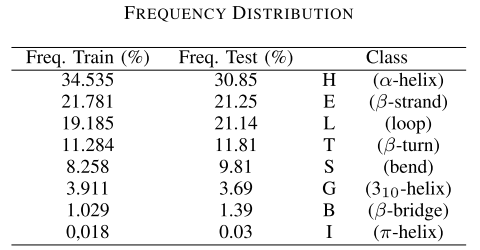
\includegraphics[width=0.5\linewidth]{targetfreq}
	\caption{Target frequencies on the CB6133 (left) and the CB513 (right).}
	\label{fig:targetfreq}
\end{figure}


\section{Network of study}\label{sect:network}

"developed by Jurtz \textit{et al} \cite{Jurtz2017} on the \textit{Lasagne} framework, which can be easily downloaded from their GitHub repository\footnote{https://github.com/vanessajurtz/lasagne4bio}. In their work, they hold a deep learning approach to solving the labelling problem, reaching an accuracy above the previous state-of-the-art (70,2\%~Q8).
[...]
Cross-entropy is used as the cost function and an L2 regularization term is included as well.
[...]
For my algorithm, I have used the code from the web as a frame (for fetching and formatting the training and test set, as well as for training and evaluation).
[...]
Batch normalization~\cite{Ioffe2015} is applied in the first dense layer, between the linear combination and the non-linear operator. Parameters of the dense and convolutional layers are initialized with uniform glorot initialization~\cite{Glorot2010}, [...] and biases to zero. Training occurs with mini-batches of 64 sequences (reshuffled after each epoch), and the update follows the RMSprop rule, with the learning rates of each parameter being dynamically adapted. Training is carried out on 5278 sequences from the training set and the remaining 256 are reserved for choosing the best epoch (validation)." [My homework]

"where a single protein sequence has an average length of roughly 214 amino acid residues." \cite{Busia2017}

My own network (simple)
Three convolutional layers, with filters of size 3, 5 and 7, and 16 filters per size
Skip connections from all previous layers (a la ResNet)
Total window size: 19 (9 per side)

With the new model all saliencies can be calculated in 3 days (as compared to the 240 days of the previous model)
"the validation set was used to pick the weights from the best performing epoch" \cite{Jurtz2017}

Iridis5 CITE

\subsection{Local and non-local interactions}
"This suggests that a large portion of the information relevant to predicting an amino acid’s secondary structure arises from the local interactions amongst relatively few of the directly neighboring residues, with the recurrent layers in Li \& Yu (2016) model learning relatively little additional information from the remainder of the input sequence." \cite{Busia2017}

"It is well known that local contexts are critical for protein secondary structure prediction. Specifically, the secondary structure category information of the neighbours of an amino acid are the most effective features for classifying the secondary structure this amino acid belongs to. [...] On the other hand, long-range interdependency among different types of amino acids also holds vital evidences for the category of a secondary structure, e.g., a β−strand is steadied by hydrogen bonds formed with other β−strands at a distance [Zhou and Troyanskaya, 2014]." \cite{Li2016}

\subsection{Window size}
"We fix the window size to 11 because the average length of an alpha helix is around eleven residues58 and that of a beta strand is around six59" \cite{Wang2016}

\subsection{Framework}
"With the recent booming of deep learning, there has also been a steady growth of programming frameworks that dramatically simplify the design and development of deep learning tools. With no single framework dominant over the others, the choice can be made based on the programming language that serves as interface or specific characteristics that each of them has. Popular frameworks nowadays are \textit{Caffe}, \textit{Theano}, \textit{Torch}, and \textit{Tensorflow}. A list of them along with their characteristics can be found in~\cite{Ravi2017}. Open-sourcing the code is a common practice in bio-medical research, and therefore there are a lot of examples available on public repositories such as \textit{GitHub}." [My lit review]

"The successes of neural networks have led to the development of various programming frameworks to build and train neural net- works. Examples are PyTorch (http://pytorch.org/), Caffe (http:// caffe.berkeleyvision.org) and TensorFlow (https://www.tensorflow.org). Our framework of choice here is Lasagne (Dieleman et al., 2015), a well-established easy to use and extremely flexible light- weight Python library built on top of the Theano numerical compu- tation library (Bastien et al., 2016). While most other frameworks require the user to learn a dedicated programming language, Lasagne is Python-based and therefore relatively easy to use for bio- informaticians already programming in Python. Further Lasagne’s active community ensures that the latest neural network training al- gorithms and architectures are available to the user." \cite{Jurtz2017}

"TensorFlow 1.0 (Abadi et al., 2016) and Keras 2.0 (Chollet, 2015; https://github.com/fchollet/keras) were used for the training of the deep learning." \cite{Fang2017}

"The software was developed using the Python programming language and the Lasagne framework 3." \cite{Hattori2017}

"We use Google’s open-sourced TensorFlow library (Abadi et al., 2016) to implement and train our networks." \cite{Heffernan2017}

"Our models are implemented using TensorFlow, an open-source machine learning software library available at TensorFlow.org." \cite{Busia2017}

	\subsubsection{Lasagne}
	"Lasagne is a lightweight library to build and train neural networks (Dieleman et al., 2015). It is written in the Python programming language (Python Software Foundation, Python Language Reference, version 2.7) and built on top of another library called Theano (Bastien et al., 2012), which allows the user to define, optimize and evaluate mathematical expressions and most importantly for neural network training it implements efficient symbolic differentiation. Another key advantage of Theano, which is also inherited by Lasagne, is that it makes using a GPU easy and transparent.
	
	Lasagne is being constantly updated, providing its users with an easy way to implement and test the newest neural network architectures and training procedures. At the time of writing, the Lasagne library contains feed forward, convolutional and recurrent layers, various activation functions and many options for weight initialization and gradient descent optimizers including Nesterov momentum, RMSprop and ADAM (Kingma and Ba, 2014). 
	
	The Lasagne documentation includes a tutorial and other code examples in a recipe directory." \cite{Jurtz2017}

\section{Feature visualization}
First order filters. They only show the first layer of feature extraction.
Optimization maximization. Bound to give unreal data. Not credible priors.


\section{Saliency maps}

Previous techniques apply to whole sequence (they were many-to-one and not many-to-many). Needs for methods of aggregating saliencies.

Using gradient * input because of simpleness. Could be further expanded to DeepLIFT

	\subsection{Analysing saliencies}
	Talk about dimensions: saliency value, class, sequences, positions, window, amino-acids, aa/pssm (7 dimensions). From now on, individual saliency maps will refer to the saliency map of one sequence-position
	
	Per-sample saliency map
	Saliency map aggregation: because many-to-many. How to do?
	
	Problems with saliency aggregation %INclude my plots with the sliding saliencies
	On the right, saliencies of subsequent single positions. Each line of a plot represents one aminoacid. Each plot corresponds to one position. X axis is the window size (19)
	Motifs slide through the saliencies, which makes:
	Sheer aggregation to capture the sliding effect
	Clustering of full saliencies useless 
	
	Solution:
	By aggregating each saliency on its window length (right), the motifs are preserved %INclude my plots with the sliding window aggregations
	Clustering on the saliencies (cosine) in the positions with high prediction for one class can show different kinds of motifs that activate that class
	 
		\subsection{Clustering on saliencies}
		Using the per-class window-aggregated version of individual saliency maps (4 dimensions left)
		Cosine distance metric.
		Show either all profiles per-cluster (3 dimensions), or aggregated profiles (2 dimensions)

\section{Open-source}
"We developed the first open-source deep-learning based secondary structure prediction tool MUFold-SS. It was implemented and provided to the research community. The open source advantage adds significant value to this work, as it allows other researchers to easily apply this deep-learning framework for many other research problems." \cite{Fang2017}